\documentclass[11pt,runningheads,oribibl]{llncs}
%
\usepackage{amsmath}
\usepackage{breqn}
\usepackage[table]{xcolor}
\usepackage{graphicx}
% Used for displaying a sample figure. If possible, figure files should
% be included in EPS format.
%
\usepackage{natbib}
\renewcommand\bibsection{\section*{\refname}}

\usepackage[hyphens]{url}
\usepackage[breaklinks]{hyperref}
\renewcommand\UrlFont{\color{blue}\rmfamily}

\begin{document}
%
\title{A Synthetic Supplemental Public Use File Of Low-Income Information Return Data: Methodology, Utility, and Privacy Implications}
%
\titlerunning{Synthetic Supplemental Public Use File}

\author{Claire McKay Bowen\inst{1} \and %\orcidID{0000-0002-1020-3181} 
Leonard Burman \inst{1,2} \and
Victoria Bryant \inst{3} \and
Surachai Khitatrakun\inst{1} \and
Philip Stallworth\inst{4} \and
Kyle Ueyama\inst{1} \and
Aaron Williams\inst{1}
}
%
\authorrunning{CMK Bowen et al.}
% First names are abbreviated in the running head.
% If there are more than two authors, 'et al.' is used.
%
\institute{Urban Institute, Washington D.C. 20024, USA \and
Syracuse University, Syracuse, New York 13244, USA \and
Internal Revenue Services, Washington D.C. 20002, USA \and
University of Michigan, Ann Arbor, MI 48109, USA}
%
\maketitle              % typeset the header of the contribution
%
\begin{abstract}
    US government agencies possess data that could be invaluable for evaluating public policy, but often may not be released publicly due to disclosure concerns. For instance, the Statistics of Income division (SOI) of the Internal Revenue Service (IRS) releases an annual public use file (PUF) of individual income tax returns that is invaluable to tax analysts in government agencies, nonprofit research organizations, and the private sector. However, SOI has taken increasingly aggressive measures to protect the data in the face of growing disclosure risks, such as a data intruder matching the anonymized public data with other public information available in nontax databases. In this paper, we describe our approach to generate a fully synthetic representation of the income tax data by using sequential Classification and Regression Trees (CART) and kernel density smoothing. This synthetic data file represents previously unreleased information useful for tax modeling. We also tested and evaluated the tradeoffs between data utility and disclosure risks of different parameterizations using a variety of validation metrics. The resulting synthetic data set has high utility, particularly for summary statistics and microsimulation, and low disclosure risk.\\
    
    \textbf{keywords:} disclosure control; synthetic data; utility; classification and regression trees
\end{abstract}

\section{Introduction}\label{sec:intro}

Tax data are a potentially invaluable resource for public policy analysis on a wide range of issues. The Internal Revenue Service (IRS) has for decades released a public use file (PUF) with selected information from individual income tax return records, anonymized and altered to protect against the risk of disclosure. Analysts in academia, nonprofit research organizations, and the private sector use the PUF to study the effects of tax policy changes on revenues, distribution of tax burdens, and economic incentives. For instance, the microsimulation models of other organizations, such as the American Enterprise Institute, the Urban-Brookings Tax Policy Center, and the National Bureau of Economic Research, must rely on the PUF. However, concerns about protecting the data participants’ privacy in the information age have required the IRS to limit the data released and distort the data in increasingly aggressive ways. As a result, the released data are becoming less and less useful for analysis and there is a risk that the PUF as currently conceived may no longer be produced. 
% Additionally, privacy protections are required by section 6103 of the Internal Revenue Code, which strictly limits access to tax return information and research based on tax return information. For example, statistical research to estimate taxpayer’s behavioral responses to income tax parameters, such as the response of capital gains realizations to changes in tax rates, can only be performed directly by researchers in Congressional Joint Committee on Taxation (JCT) and Treasury’s Office of Tax Analysis (OTA) or in collaboration with them, or through a highly restrictive arrangement with the IRS.

In order to improve the PUF's utility, we developed a synthetic data approach to protecting the tax data from disclosure. Although synthetic data generation has been used to protect many administrative and other sensitive data sets against disclosure, it has not previously been applied to U.S. tax data. More specifically, the 2012 Supplemental Public Use File (PUF), a database of individuals who were not dependents and did not file an individual income tax return in 2012. More information about the file is available in \cite{irs2019}. 

We organize the paper as follows. Section \ref{sec:method} details our synthetic data generation method on the Supplemental Public Use File data and outlines how our synthesis process protects privacy, including protections against disclosure of outliers and attribute disclosure. Section \ref{sec:results} reports and evaluates the data utility measures of the synthesized Supplemental Public Use File data. Further discussion of our results and our plans for future work are in Section \ref{sec:diss}.

\section{Synthesizing the Supplemental Public Use File Methodology}\label{sec:method}

Our main objective is to synthesize records from the IRS Master File to create a synthetic file similar to the current PUF released by the IRS Statistics of Income (SOI) Division, but with stronger privacy protections. As a proof of concept and in an effort to release useful data that had never before been made public, we first created a fully synthetic file called the Supplemental PUF. 

According to \cite{cilke2014case}, a nonfiler is, ``Any U.S. resident that does not appear on a Federal income tax return filed [for] a given year.'' Our sample is thus comprised of people who do not file a federal income tax return for a given year and do not appear to have an income tax filing requirement. Additionally, our data source is a random 0.1\% sample of information returns for Tax Year 2012 maintained by the IRS SOI Division. Information returns are forms provided to the IRS by any business or other entity that pays income or has certain other transactions with an individual. The following section provides background on the Supplemental PUF and outlines the disclosure risks and data synthesis process for this file.

\subsection{Background}
Data stewards (also referred to as data curators or data maintainers) have relied on a variety of statistical disclosure control (SDC) or limitation (SDL) techniques to preserve the privacy of data while maintaining quality. However, some SDC techniques may fail to eliminate disclosure risk from data intruders armed with external data sources and high-powered computers \citep{drechsler2010sampling,winkler2007examples}. These techniques may also greatly reduce the usefulness of the released data for analysis and research. For instance, currently, the IRS \textit{top codes} the number of children variable in the individual income tax return public use file (PUF) at 3 for married filing jointly and head of household returns, 2 for single returns, and 1 for married filing separately returns \citep{bryant2017general}. Also, the 2012 PUF \textit{aggregated} 1,155 returns with extreme values into four observations \citep{bryant2017general}. These methods may degrade analyses that depend on the entire distribution, bias estimates from more complex statistical models, distort microsimulation model analyses that are sensitive to outliers, make small area estimation impossible, and hide spatial variation \citep{reiter2014bayesian,fuller1993masking}. 

% For instance, \textit{adding random noise} can create measurement error in the perturbed variables, reducing the precision of statistical analyses and potentially introducing bias \citep{yancey2002disclosure}. \cite{mitra2006adjusting} found that \textit{data swapping} at a 5 percent random swapping of two identifying variables in the 1987 Survey of Youth in Custody invalidated statistical hypothesis tests in regression models that included those variables. \cite{drechsler2010sampling} also discovered that even 1 percent swapping of a subsample from the March 2000 U.S. Current Population Survey can undermine statistical inference.

\subsection{Disclosure Risks}
% Any public data release must protect the confidentiality of individual taxpayer information. Ensuring the confidentiality of a data set is challenging and complicated because more and more data that might appear on tax returns exists in other public and private databases while the computational power required to match data from different sources continues to grow. To address this challenge, we propose a data synthesis methodology that protects against meaningful disclosure. We define a meaningful disclosure as information that would allow an intruder to: (1) infer whether any individual is in or out of the underlying data set, i.e., whether they have filed a tax return, or (2) update their estimate of the range of any variable compared with the estimate ascertainable without access to the synthetic data file

Replacing actual data with fully synthetic data has the potential to avoid the pitfalls of previous SDC techniques. The approach achieves this by attempting to simulate the data generation process of the confidential data based on a model of the underlying distribution. This method protects against identity disclosure, because no real observations are released \citep{hu2014disclosure, raab2016practical}. Specifically, \cite{hu2014disclosure}, stated that ``it is pointless to match fully synthetic records to records in other databases since each fully synthetic record does not correspond to any particular individual.'' However, if not carefully designed, fully synthetic data may still risk disclosing information \citep{raab2016practical}. For example, overfitting the model used to generate the synthetic data might produce a synthetic file that is too close to the underlying data. In the extreme case, a data synthesizer could theoretically perfectly replicate the underlying confidential data (Elliot 2014). The database reconstruction theorem (Dinur and Nissim 2003) proves that even noisy subset sums can be used to approximate individual records by solving a system of equations. If too many independent statistics are published based on confidential data, then the underlying confidential data can be reconstructed with little or no error.

% To date, the only identified disclosure risks have been with respect to discrete variables and counts. Disclosure may be possible in the case of categorical variables that have a limited number of possible values because they may be solved for with a finite set of simultaneous equations and a limited amount of information. \cite{hu2014disclosure} determined re-identification risks on synthetic data in the American Community Survey. The authors calculated posterior probability distributions for categorical variables based on the method used to synthesize the data. 

Disclosure risks are difficult to estimate on complex synthetic data sets such as a synthetic individual income tax return database. \cite{raab2016practical} concluded that it was impractical to measure disclosure risk in the synthesized data from the UK Longitudinal Series: ``\cite{hu2014disclosure, reiter2014bayesian,mcclure2012differential} proposed other methods that can be used to identify individual records with high disclosure potential, but these methods cannot at present provide measures that can be used with (the) sort of complex data that we are synthesizing.'' [p. 82]

However, there are three aspects of the data and our proposed methodology that protect against disclosure: 
\begin{enumerate}
    \item The administrative databases are very large, so a substantial amount of information may be released without allowing a data intruder to infer anything useful about individuals unless they already possessed almost all the original data. Moreover, the dimensionality of the solution problem becomes quite large and computationally demanding.
    \item The synthetic data set will be only a fraction (no more than 1 in 10) of the size of the underlying administrative data.
    % We show later in the section that this protects against meaningful disclosure about the idiosyncrasies of the underlying empirical distribution. Essentially, sampling reduces disclosure risk because there is no guarantee that a targeted individual is in the sample before it is synthesized \citep{reiter2005estimating,matthews2011data}.
    \item Data intruders often have more information about outliers and may have more to gain from identifying them. Our synthetic data method smooths the distribution of underlying data, preserving the empirical distribution for non-sensitive observations. Specifically, the empirical distribution has a high population density, and then flattens in the tails to only reflect the general characteristics of the outlier observations. This protects against inference of even very sensitive observations.
\end{enumerate}

\subsection{Data Synthesis Procedure}
For our synthetic data generation process, we used classification and regression trees (CART) as our underlying model \citep{breiman1984classification,reiter2005using}. We focus on implementing CART because the method is computationally simple and flexible. Additionally, CART out-performed regression-based parametric methods in preliminary tests. We used a customized version of CART from the R package \verb;synthpop;, which contains multiple methods for creating partially-synthetic and fully-synthetic data sets and for evaluating the utility of synthetic data \citep{nowok2019package}. 

Essentially, we used CART to partition the sample into relatively homogeneous groups, subject to the constraint that none of the partitions be too small, to protect against overfitting \citep{benedetto2013creation}. In testing on the Supplemental PUF database, we found that a minimum partition size of 50 produces a good fit with adequate diversity of values within each partition. Note that the optimal size may be different when synthesizing individual income tax return data. 

\begin{dmath}
    f(X_1,X_2,...,X_k|\theta_1,\theta_2,...,\theta_k) = f_1 (X_1|\theta_1)\cdot f_2(X_2|X_1,\theta_2)...
    f_k(X_k|X_1,...,X_{k-1},\theta_k)
\end{dmath}

\noindent where $X$ is the variables to be synthesized, $\theta$ is the vector of model parameters such as regression coefficients, and $k$ is the total number of variables (19) such that $i = 1$ to $k$.

To develop the synthetic Supplemental PUF data set, we first split the data into two parts. One part includes the observations from the confidential data that have zeros for all seventeen tax variables. The other part includes the observations with at least one non-zero tax variable. For the part with all zeros for tax variables, we randomly assign the \textit{gender} value based on the proportions in the zero subsample, synthesize \textit{age} based on \textit{gender}, and assign zeros to all tax variables. 

For the part with at least one non-zero value for a tax variable, we randomly assign \textit{gender}, $X1$, values based on the underlying proportions in the confidential data set. With 51 percent female and 49 percent male in the administrative data set, the assigned \textit{gender} value for each row in the synthetic data set will have a 51 percent probability of female and a 49 percent probability of male. Due to the random assignment of \textit{gender}, the exact proportion of males and females in the synthetic data set may differ slightly from the distribution of \textit{gender} in the administrative data, but the difference is likely to be small given the sample size. 

We then use CART to assign \textit{age}, $X_2$, to each record conditional on \textit{gender}. Since the CART method selects values at random from the final nodes, the distribution may differ slightly from the distribution of \textit{age} by \textit{gender} in the administrative data, but the differences are likely to be small given the sample size. \textit{Age} is top coded at 85 after synthesis. To measure heterogeneity, the algorithm in our synthesis uses a Gini index.

\begin{equation}
    I(A)=\sum_{i=1}^C p_i (1-p_i)
\end{equation}

\noindent where $A$ is a node, $C$ is the number of classes in the node (e.g. 2 for binary \textit{gender}), and $p_i$ is the class probability for the $i$th class (e.g., 0.51 are Female). The best split minimizes 

\begin{equation}
    \frac{N_L}{N}I(A_L)+\frac{N_R}{N}N(A_R)
\end{equation}

\noindent where $N_L$ and $N_R$ are the number of observations in the left and right nodes created by the split respectively, $N= N_L+N_R$ is the total number of observations in both nodes, and $I(A_L)$ and $I(A_R)$ are the Gini index in the left and right nodes, respectively. Splits continue until there is no reduction in the heterogeneity or until the minimum size (50) for a final node is reached. 

For continuous variables, we start with the variable with the most non-zero values—\textit{wage} income, $X_3$, and then order the remaining variables, $\{X_4, X_5,..., X_19\}$, in terms of their correlations with \textit{wage}, from most highly to least correlated. Specifically, at each partition, the ``best split'' is the one that minimizes the error sum of squares, $SSE$, given that the data are partitioned into two nodes. Thus, 

\begin{equation}
    SSE=\sum_{i\in A_L}(y_i-\bar{y}_L)^2 + \sum_{i\in A_R}(y_i-\bar{y}_R)^2
\end{equation}

\noindent where $A_L$ and $A_R$ are the left and right nodes created by the split. The variables $\bar{y}_L$ and $\bar{y}_R$ are the means of the left and right nodes respectively \citep{kuhn2013applied}. Splits continue until there is no improvement in the splitting criteria or until the minimum size for a final node is reached (50). Our data synthesis approach samples values from the appropriate final node and then applies our smoothing method. 

To synthesize the first continuous variable $X_3$, (\textit{wages} in the Supplemental Public Use File data), we create a smoothed kernel density function for each percentile of values predicted by CART for this variable. As shown in Figure \ref{fig:kde}, the kernel density estimator is the aggregation of individual normal densities centered around each observation \citep{wicklin2016visualize}. In the example, each of the individual Gaussian kernels has the same variance. The kernel density distribution is smooth and unbounded. 

However, we must tackle some complications with executing this approach. First, the variance of the Gaussian kernel must be larger when sampling outliers. If the variance was not larger, a data intruder who knows how the database is constructed might draw some fairly precise inferences since outlier observations in the synthetic data set would likely be relatively close to an actual observation. We use percentile smoothing, which selects the variance based on the optimal variance for a kernel density estimator estimated on observations in the percentile for each observation. As discussed later in the section, this causes the variance to grow with the value of the synthesized variable. Secondly, variables that are a deterministic function of others, such as adjusted gross income or taxable income, will be calculated as a function of the synthesized variables. We do not calculate such variables for the Supplemental PUF data.

\begin{figure}
    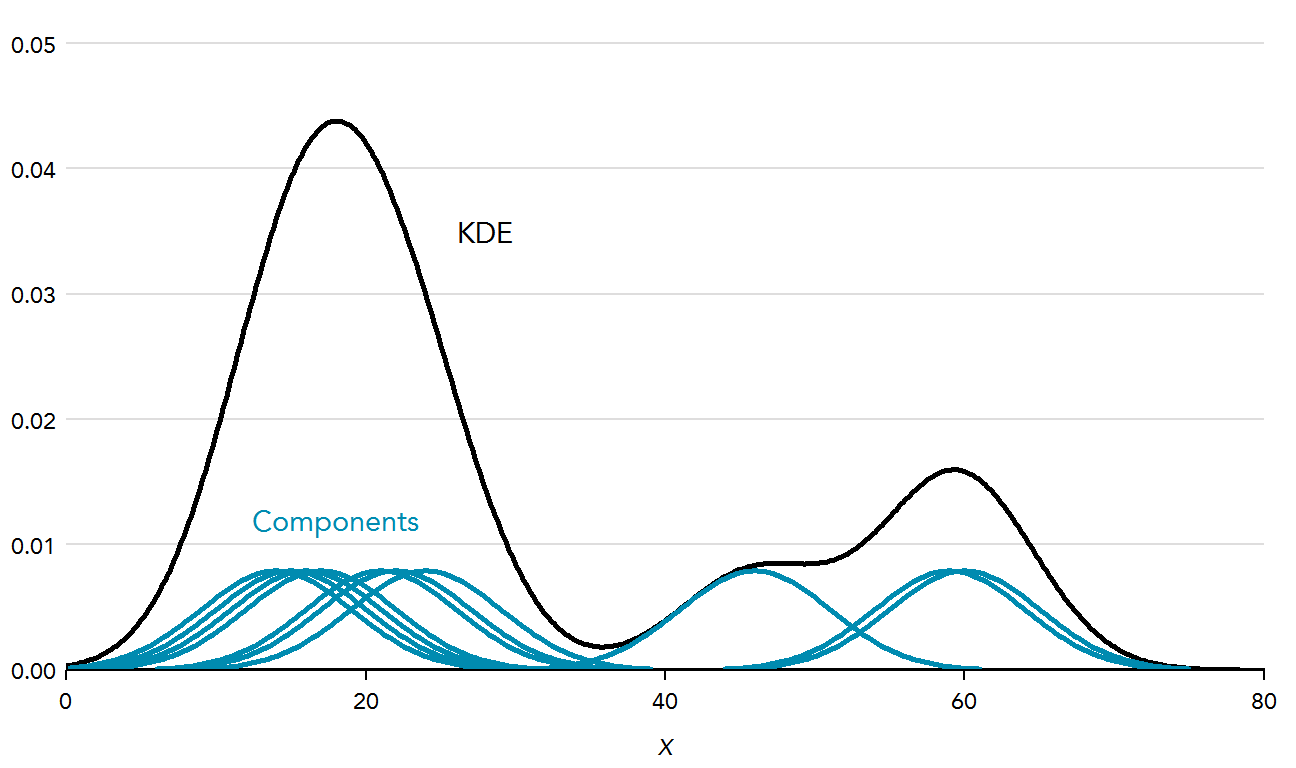
\includegraphics[width=\textwidth]{figures/kde-1.png}
    \caption{Kernel Density Estimate as Weighted Sum of Component Densities.} \label{fig:kde}
\end{figure}

No smoothing is applied to values of 0, which is the most common value for all continuous variables in the Supplemental PUF data. We do not consider zeros to be a disclosure risk because the variable with the most non-zero values still contains 73 percent zeros. Many of the variables are zero for almost every record. By default, \verb;synthpop; does not smooth values if the frequency of a single value exceeds 70 percent. 

Subsequent variables $\{X_4, X_5,..., X_19\}$ (all the tax variables) are synthesized in a similar way to $X_3$ by using CART to predict values based on random draws from the kernel density estimator of observations with similar characteristics. Classification trees and regression trees for prediction tend to over-fit data, therefore most trees are reduced based on a penalty for the number of final nodes in the tree \citep{kuhn2013applied}. For the Supplemental Public Use File we did not reduce trees because our minimum partition size is large (50).

\subsection{Measurement of the Privacy Protection}
Our data synthesis methodology is designed to protect confidentiality ex ante, but we also used a set of privacy metrics to test whether the CART method might produce values that are too close to actual values or reveal too much about relationships between variables. We used these metrics to adjust the precision of the data synthesis by adjusting smoothing methods and parameters such as the minimum size of the final nodes in the CART synthesizer. 

\subsubsection{Duplicates:} We examined several metrics for the frequency and uniqueness of synthesized rows in the confidential data. Even though all non-zero values are individually synthesized, it is possible that a row in the synthetic data can match a row in the confidential data by chance. The simplest metric of duplication is a count of rows in the unsmoothed synthetic data that match rows from the confidential data–but this is not particularly informative for two reasons. First, many rows have values for \textit{age}, \textit{gender}, and then all zeros for the tax variables. The probability of duplicating these rows is high but does not carry any disclosure risk. Second, there are many rows that occur in the confidential data that would be expected to appear as replicated in the confidential data by chance. 

\subsubsection{Number of unique-uniques:} The count of unique-uniques is the number of unique rows from the confidential data that are unique in the unsmoothed synthetic data. This narrows the focus to rows that are uncommon and could carry some inferential disclosure risk.  

\subsubsection{Row-wise Squared Inverse Frequency:} Finally, we used a measure based on frequency. For any given row in the unsmoothed synthetic data, this metric counts the number of identical rows in the confidential data. We then take the inverse square of this metric such that rows that appear once are assigned a value of 1, rows that appear twice are assigned a value of 1/4, rows that appear thrice are assigned a value of 1/9, and so on. 

\subsubsection{$l$-diversity of final nodes in the CART algorithm:} We were concerned that the CART algorithm could generate final nodes that lack adequate heterogeneity to protect confidentiality. Too little heterogeneity in the final nodes could result in too much precision for the synthesizer. To ensure adequate heterogeneity, we applied $l$-diversity to the decision trees created by the CART algorithm \citep{machanavajjhala2007diversity}. Let a quasi-identifier be a collection of non-sensitive variables in a data set that could be linked to an external data source. Let a $q^*$-block be a unique combination of the levels of quasi-identifiers. A $q^*$-block is $l$-diverse if it contains at least $l$ unique combinations of sensitive variables. We applied this formal measure to the CART algorithm, where at each partition the split directions (left and right) are considered to be quasi-identifiers and the final nodes are considered to be $q^*$-blocks. The trees create the discretized space formed by quasi-identifiers, the final nodes are $q^*$-blocks, and the sensitive values are the values in the final nodes. We examine the minimum $l$-diversity in a data synthesizer and the percent of observations that came from final nodes with $l$-diversity less than 3. In many cases, the minimum $l$-diversity is 1 because some final nodes only contain zeros. We consider this to be acceptable because zeros carry negligible disclosure risk.

\section{Data Quality and Evaluation of the Synthetic Supplemental Public Use File Data}\label{sec:results}

\begin{figure}
    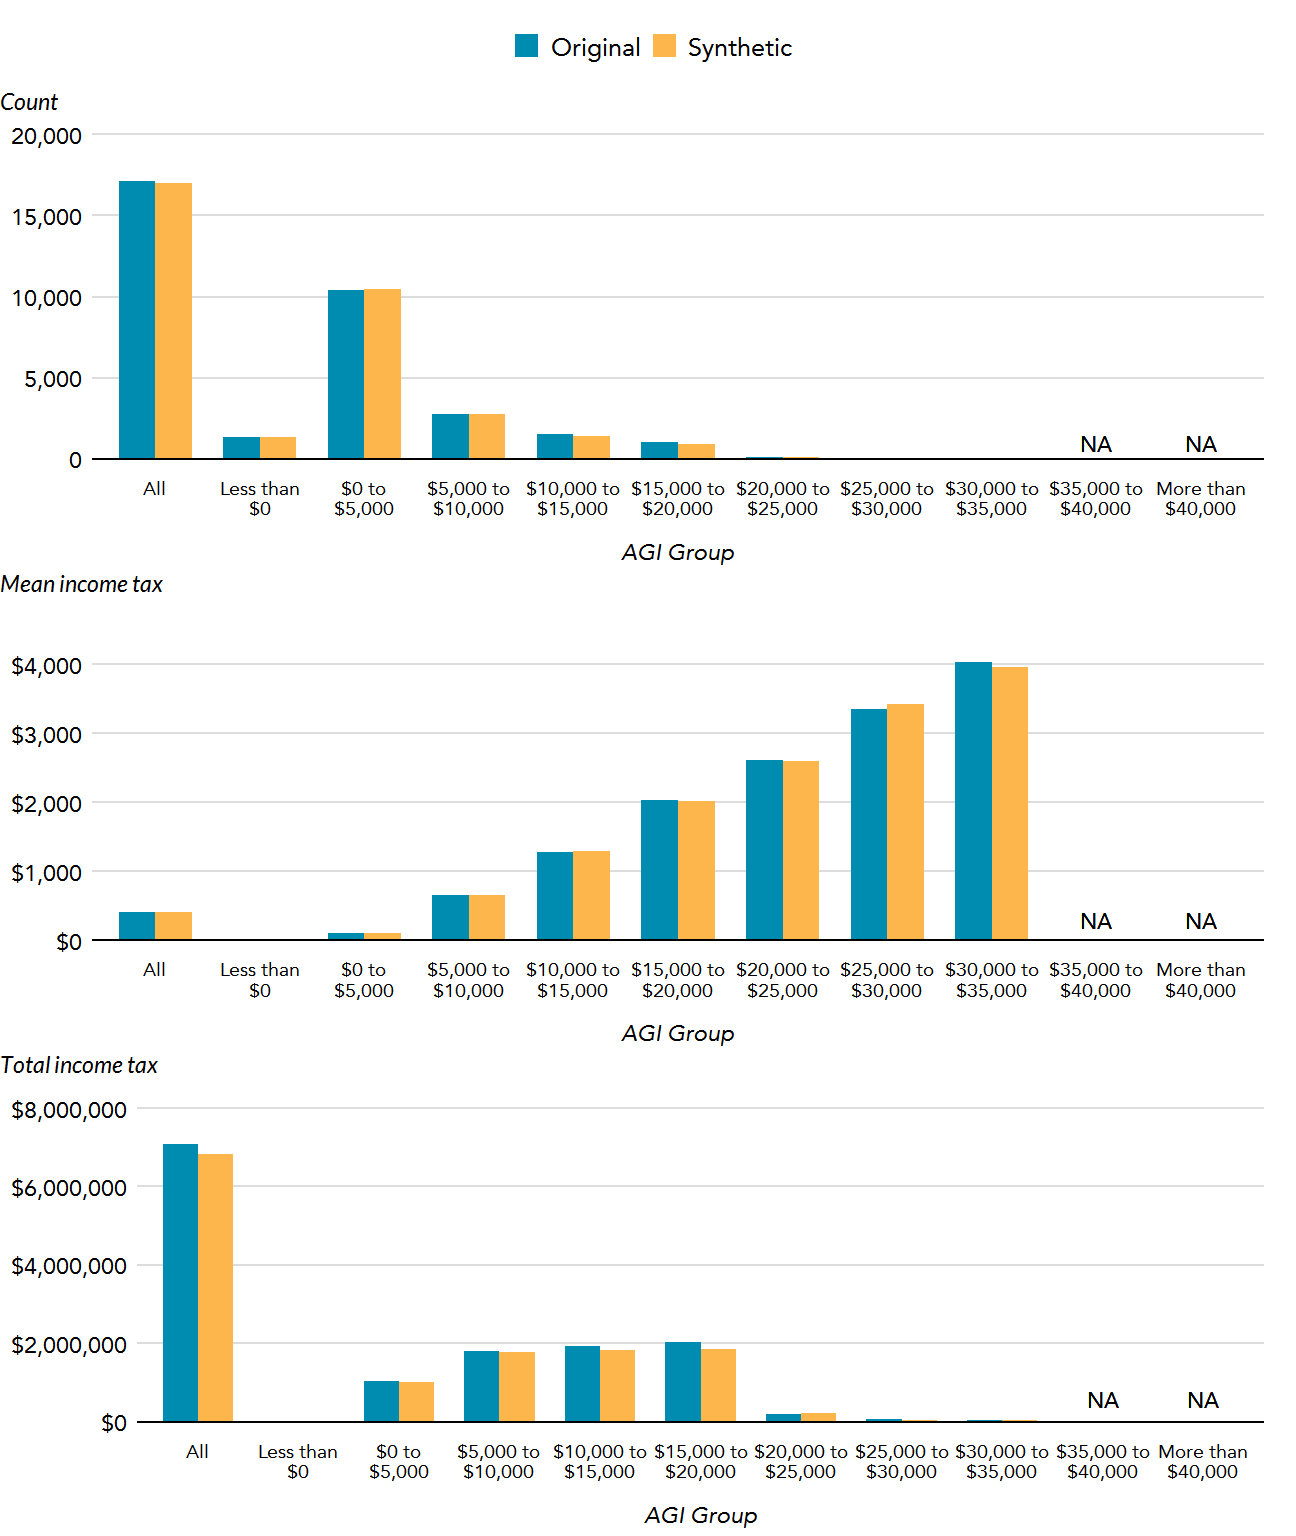
\includegraphics[width=\textwidth]{figures/tax-calulator-1.png}
    \caption{Tax Calculator Results for the original and synthetic Supplemental PUF data.} \label{fig:tax}
\end{figure}

In this section, we report the utility results of the synthetic Supplemental PUF. We first compared several summary statistics for the seventeen tax, which included the means and standard deviations. Figures \ref{fig:mean} and \ref{fig:sd} in the Appendix shows that original and synthetic \textit{age} and the 17 tax variables had similar values overall. A few variables differed a lot such as the standard deviation of \textit{tax-exempt interest} and the kurtosis of \textit{above the line}.

We also examined the correlation fit, where the correlation fit was 0.0013 across all variable. Figure \ref{fig:corr} in the Appendix illustrates the correlation difference between every combination of tax variables. Most differences are close to zero. \textit{Taxable dividends}, \textit{qualified dividends}, \textit{tax-exempt interest}, and \textit{long-term capital gains} all have correlation differences that are not close to zero. This is not surprising since these variables have very few non-zero values and are uncommon sources of income for nonfilers. We do not consider this a cause for concern, but it is an area for future improvement.

We applied pMSE, a propensity-score-based utility measure, that tests whether a model can distinguish between the confidential and the synthetic data. \cite{woo2009global} introduced and \cite{snoke2018general} enhanced a propensity score measure for comparing distributions and evaluating the general utility of synthetic data. We used a logistic regression with only the main effects, resulting in a p-value of the pMSE as 0.26. This suggests the model had difficulties distinguishing between the confidential and synthetic Supplemental PUF. 

Ultimately, the synthetic Supplemental PUF data set will be used for tax microsimulation. We built a tax calculator to compare calculations of Adjusted Gross Income (AGI), personal exemptions, deductions, regular income tax, and tax on long-term capital gains and dividends based on the confidential data and the synthetic data. The tax calculator uses a simplified version of 2012 law, the year of the confidential and synthetic data. The calculator assumes that all individuals are single filers and does not include any tax credits, standard or itemized deductions, or lowers the personal exemption to \$500. This unorthodox combination of rules is necessary to obtain useful calculations using the Supplemental PUF data, which came from a population that pays federal income tax only through withholding by payers of wages and other income. 

Figure \ref{fig:tax} compares results for the original and synthetic data sets across different AGI groups for count, mean tax, and total tax. Overall, the synthetic Supplemental PUF performs well on our simple tax calculator and approximates the results from the confidential data set.

\section{Conclusions and Future Work}\label{sec:diss}
In this paper, we developed and evaluated a method to create a fully synthetic version of the IRS Supplemental Public Use File database. We demonstrated that the synthetic data set would not allow a data intruder with extensive knowledge to meaningfully update his or her prior distribution about any variable on a tax return or even about whether someone had or had not filed a tax return beyond statistical relationships between variables. Additionally, our method generated a synthetic data set that replicates the characteristics of the underlying administrative data while protecting individual information from disclosure.

For future work, we will develop a synthetic data set based on the much more complex and diverse individual income tax return data. We do not know, a priori, how well the data synthesis methodology used for the Supplemental Public Use File data will replicate the underlying distributions of these data. For instance, we found that random forests performed worse than CART for the Supplemental Public Use File data, but random forests might outperform CART for the individual income tax return data. We plan to test a range of data synthesis methods. At a minimum, our goal is to create a synthetic file that protects the privacy of individuals and reproduces the conditional means and variances of the administrative data. The synthetic data should also be useful for estimating the revenue and distributional effects of tax law changes and for other exploratory statistical analysis. 

Experience suggests that the synthetic data will not provide accurate estimates for complex statistical models, so a key component of this project is to create a way for researchers to run their models using the actual administrative data with parameter estimates altered to protect privacy and standard errors adjusted accordingly. Other future work includes developing and establishing a validation server, a secure process to analyze the raw confidential data. This is a natural complement to the synthetic data because researchers could use the synthetic data, which have the same record layout as the confidential data, for exploratory analysis and to test and debug complex statistical programs. \citet{abowd2008protective} describe a system that provides access to the confidential version of the Survey of Income and Program Participation and receive statistical output after a privacy review by a US Census Bureau staff. Our goal is to create a similar system that would modify statistical outputs to guarantee privacy and preserve the statistical validity of estimates without requiring human review. 

\subsubsection{Acknowledgments:}
We are grateful to Joe Ansaldi, Don Boyd, Jim Cilke, John Czajka, Rick Evans, Dan Feenberg, Barry Johnson, Julia Lane, Graham MacDonald, Rob McClelland, Shannon Mok, Jim Nunns, James Pearce, Kevin Pierce, Alan Plumley, Daniel Silva-Inclan, Michael Strudler, Lars Vilhuber, Mike Weber, and Doug Wissoker for helpful comments and discussions.

This paper relies on the analytical capability that was made possible in part by a grant from Arnold Ventures. The findings and conclusions are those of the authors and do not necessarily reflect positions or policies of the Tax Policy Center or its funders.

% \newpage
% ---- Bibliography ----

\bibliographystyle{splncsnat}
\bibliography{ref}

\section*{Appendix}
The appendix contains the supplementary materials to accompany the paper ``A Synthetic Supplemental Public Use File Of Low-Income Information Return Data: Methodology, Utility, and Privacy Implications'' with additional results from the utility evaluation.

Figures \ref{fig:mean} and \ref{fig:sd} show the means and standard deviations, respectively, from the original and synthetic supplemental PUF data for \textit{age} and all seventeen tax variables. Figure \ref{fig:corr} displays the correlation differences of the synthetic data minus the original data for all seventeen tax variables.

\begin{figure}
    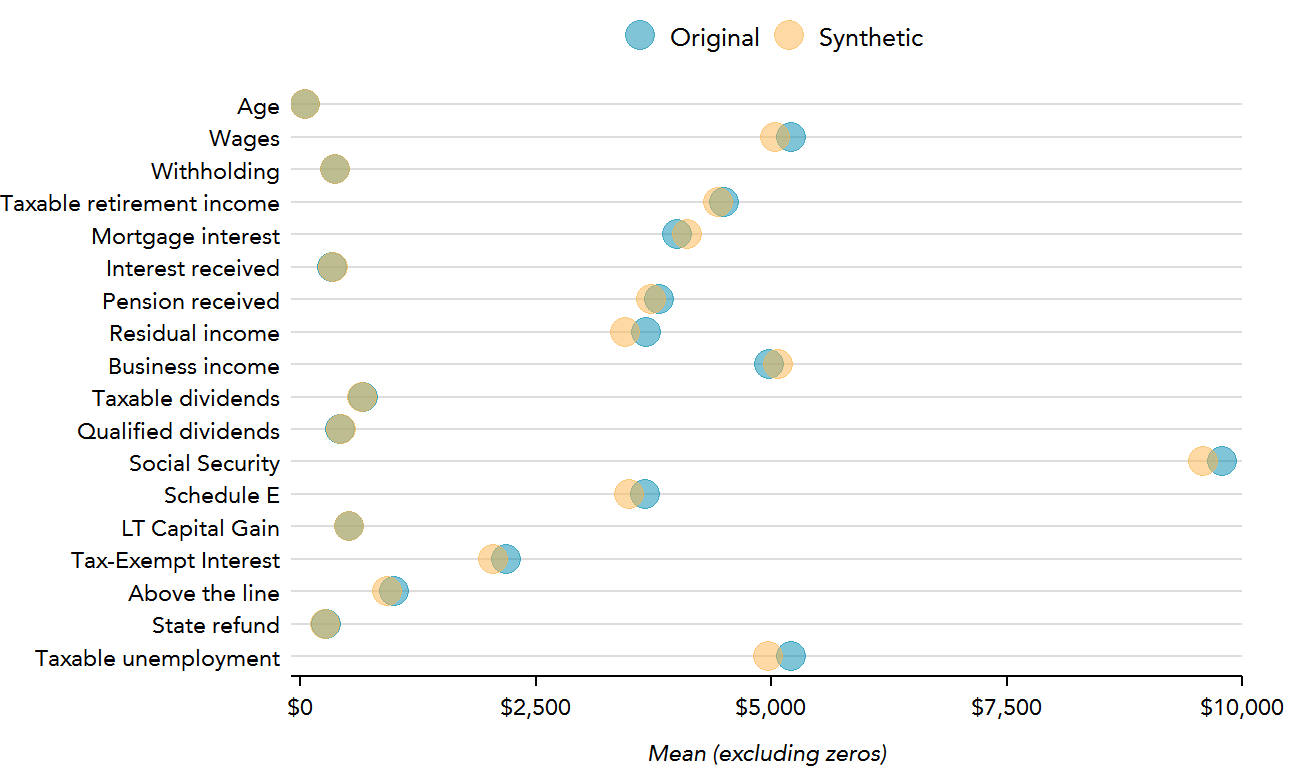
\includegraphics[width=\textwidth]{figures/means-1.png}
    \caption{Means from the original and synthetic Supplemental PUF data.} \label{fig:mean}
\end{figure}

\begin{figure}
    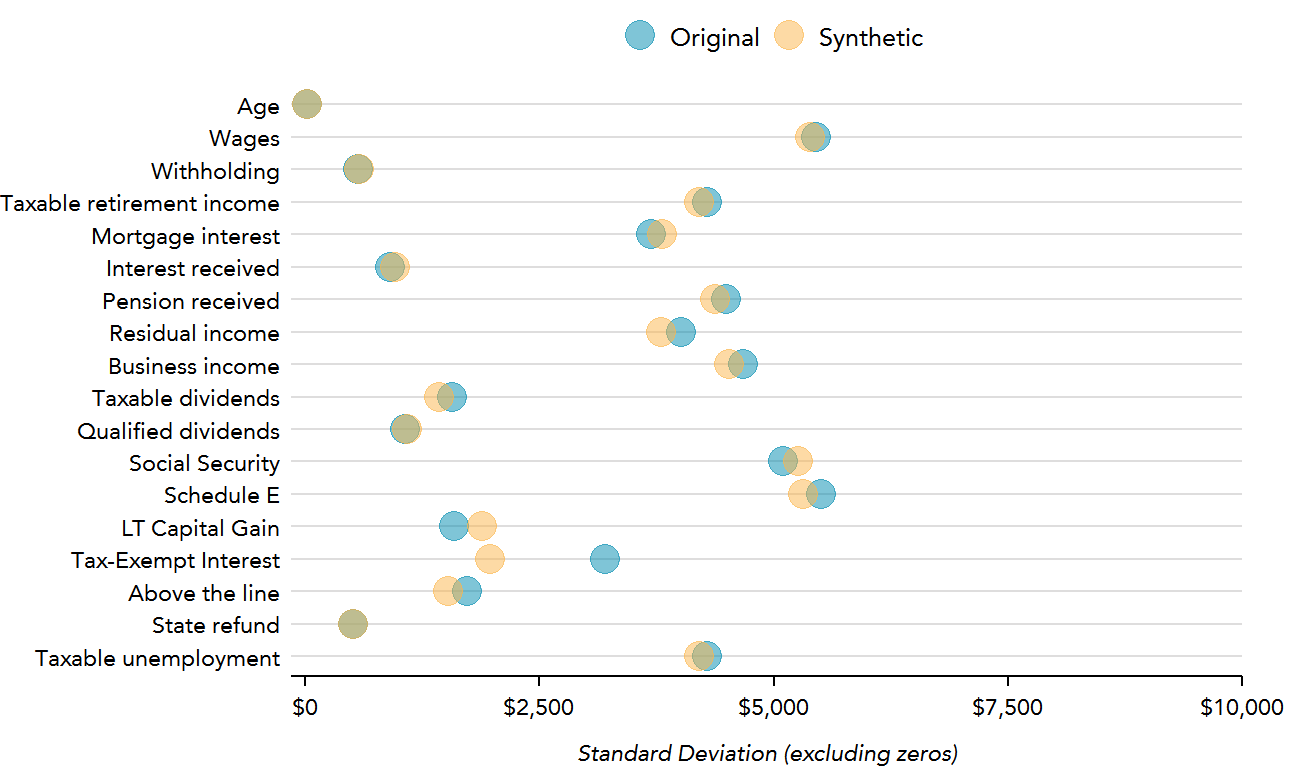
\includegraphics[width=\textwidth]{figures/standard-deviation-1.png}
    \caption{Standard Deviations from the original and synthetic Supplemental PUF data.} \label{fig:sd}
\end{figure}

% \begin{figure}
%     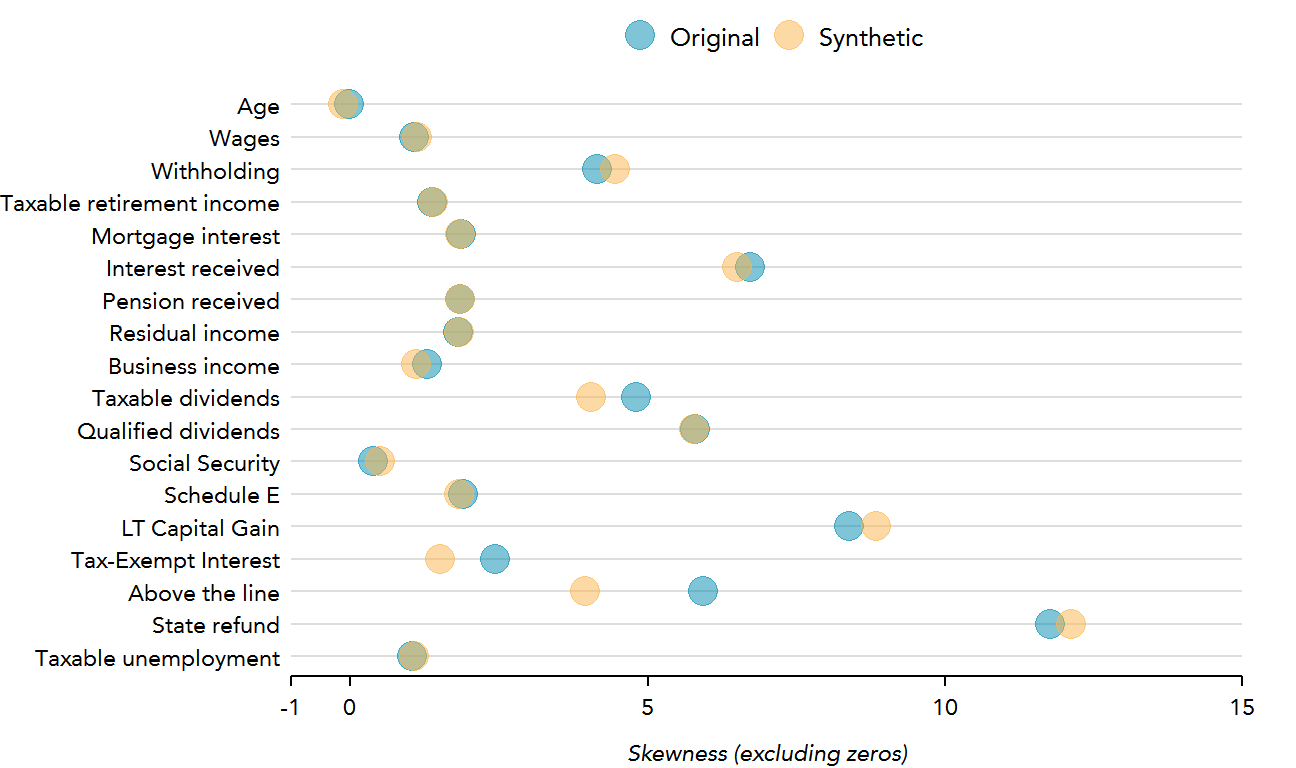
\includegraphics[width=\textwidth]{figures/skewness-1.png}
%     \caption{Skewness from the original and synthetic Supplemental PUF data.} \label{fig:skew}
% \end{figure}

% \begin{figure}
%     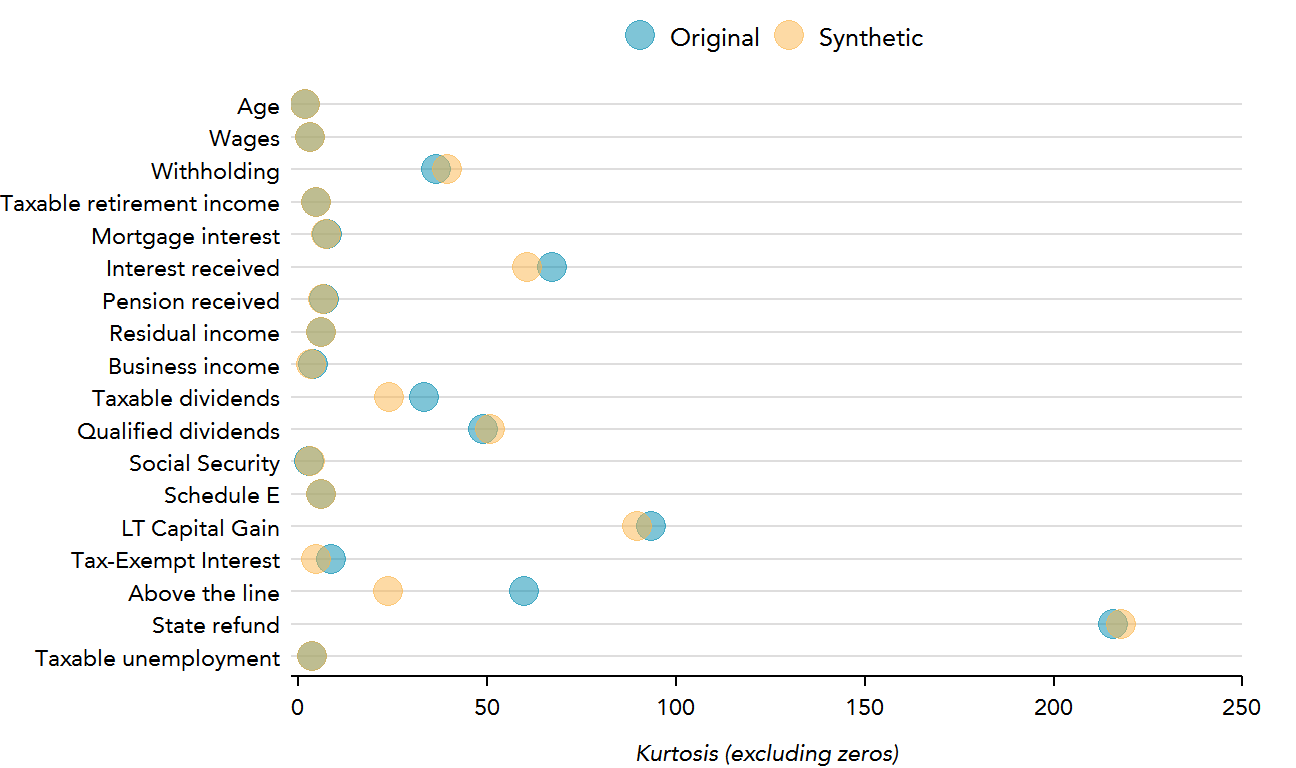
\includegraphics[width=\textwidth]{figures/kurtosis-1.png}
%     \caption{Kurtosis from the original and synthetic Supplemental PUF data.} \label{fig:kurtosis}
% \end{figure}

\begin{figure}
    \begin{center}
        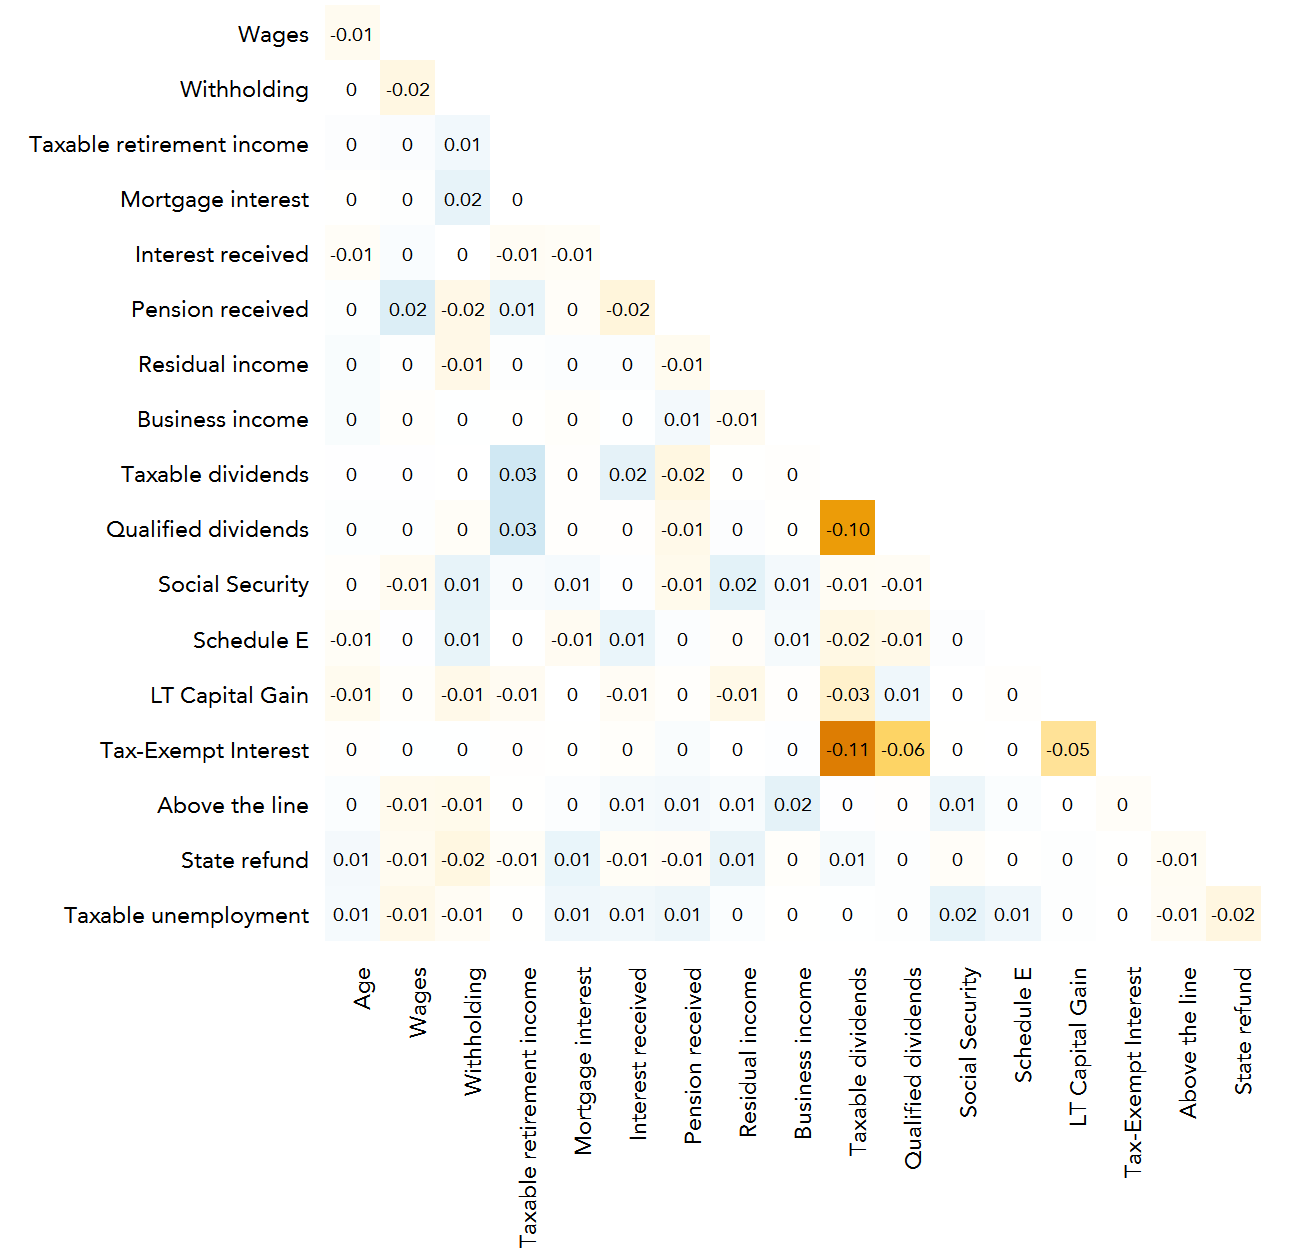
\includegraphics[width=0.8\textwidth]{figures/correlation-fit-1.png}
        \caption{Correlation differences (synthetic minus original Supplemental PUF data). Calculation excludes rows with zeros for all seventeen tax variables.} \label{fig:corr}
    \end{center}
\end{figure}



\end{document}
